\documentclass[12pt,a4paper]{article}
\usepackage[utf8]{inputenc}
\usepackage[T1]{fontenc}
\usepackage{lmodern}
\usepackage{geometry}
\geometry{left=2.5cm,right=2.5cm,top=2.5cm,bottom=2.5cm}
\usepackage{amsmath,amssymb,amsthm,mathtools}
\usepackage{bm}
\usepackage{booktabs}
\usepackage{hyperref}
\usepackage{xurl}
\usepackage{natbib}
\usepackage{graphicx}
\usepackage{xcolor}
\usepackage{tikz}
\usepackage{pgfplots}
\pgfplotsset{compat=1.18}
\usetikzlibrary{positioning,arrows.meta}

% ----------------------------------------------------------------
% YUCT‑specific macros
% ----------------------------------------------------------------
\newcommand{\Keff}{K_{\mathrm{eff}}}
\newcommand{\Dir}{\mathcal{D}}
\newcommand{\Mpl}{M_{\mathrm{Pl}}}
\newcommand{\Lpl}{l_{\mathrm{Pl}}}
\newcommand{\tP}{t_{\mathrm{P}}}
\newcommand{\Sodd}{S_{\mathrm{odd}}}
\newcommand{\Seven}{S_{\mathrm{even}}}
\newcommand{\kappac}{\kappa_{c}}
\newcommand{\betaf}{\beta}
\newcommand{\lagr}{\mathcal{L}}
\newcommand{\dint}{D\!+\!I\!\cdot\!R}
\newcommand{\CCU}{\text{CCU}}  % Cubic Coordination Unit

% ----------------------------------------------------------------
\title{\bfseries Solving Fermi's Paradox within the Yakushev Unified
	Coordination Theory: \\ From K2-18b to the Great Silence}
\author{Alexey V. Yakushev\textsuperscript{1} \\
	\small \textsuperscript{1}Yakushev Research, \url{https://yuct.org/} \\
	\small \url{https://ypsdc.com/}}
\date{June 2026}

\begin{document}
	\maketitle
	
	\begin{abstract}
		The recent detection of dimethyl sulfide (DMS) in the atmosphere of the
		exoplanet K2-18b at a concentration thousands of times higher than
		Earth's provides an unprecedented empirical anchor for the density of
		life in the cosmos.  Assuming --- in accordance with the principle of
		mediocrity --- that the volume around the Sun containing two living
		planets (Earth and K2-18b) is typical, we extrapolate the local
		density of inhabited worlds to the entire observable universe and
		obtain $N_{\mathrm{life}} \sim 10^{26}$.  Even after subtracting the
		small fraction of space sterilised by gamma-ray bursts, active
		galactic nuclei, and supernovae, the number remains astronomically
		large, exacerbating Fermi's paradox.  Within the Yakushev Unified
		Coordination Theory (YUCT) this paradox is resolved by two
		fundamental coordination thresholds: (i)~the critical efficiency for
		the emergence of self-replicating life ($K_{\mathrm{crit}}\approx150$)
		and (ii)~the inevitable transition of a technological civilisation
		into a cognitively self-sufficient, decoupled d-YPSDC state that
		renders it invisible to external observers.  Our analysis therefore
		transforms the ``Great Silence'' from a speculative puzzle into a
		quantitative, empirically grounded confirmation of the coordination
		paradigm.
	\end{abstract}
	
	% ----------------------------------------------------------------
	\section{Introduction}
	% ----------------------------------------------------------------
	The question ``Where is everybody?'' has haunted science for over
	seven decades.  Traditional attempts to solve Fermi's paradox within
	the Drake equation framework suffer from irreducible uncertainties in
	each of its probabilistic factors.  The Yakushev Unified Coordination
	Theory (YUCT) offers a radically different perspective: every step of
	cosmic evolution, from galaxy formation to the rise of consciousness,
	is governed by a single measurable parameter --- the coordination
	efficiency $\Keff$.  Consequently, the transition from a living planet
	to a technologically visible civilisation is not a chain of random
	events but a deterministic sequence of critical coordination
	thresholds.
	
	Recently, the James Webb Space Telescope detected dimethyl sulfide
	(DMS) in the atmosphere of the exoplanet K2-18b, a sub-Neptune located
	124 light-years from the Sun.  The observed concentration is orders of
	magnitude above the terrestrial background, suggesting a biosphere of
	extraordinary productivity.  This discovery provides, for the first
	time, a direct observational lower bound on the cosmic density of life.
	
	In this article we combine the K2-18b data with the YUCT framework to
	derive a robust, quantitative resolution of Fermi's paradox.  We
	proceed as follows:  Section~2 extracts the local density of inhabited
	worlds.  Section~3 extrapolates this density to the whole observable
	universe.  Section~4 discusses the astrophysical hazards capable of
	sterilising large regions.  Section~5 reformulates the problem in terms
	of the fundamental coordination volume of the universe.  Section~6
	introduces the two YUCT Great Filters and shows that they jointly
	account for the observed silence.  Section~7 provides observational
	templates to search for coordinated biospheres and technospheres.
	Section~8 presents the equation of silence, and Section~9 summarises
	our conclusions.
	
	% ----------------------------------------------------------------
	\section{The Empirical Density of Life}
	\label{sec:empirical}
	% ----------------------------------------------------------------
	Let $R_{\mathrm{life}} = 124$ light-years be the distance to the
	nearest exoplanet with a confirmed biosignature.  Inside the sphere of
	radius $R_{\mathrm{life}}$ centred on the Sun we now know of two living
	planets: Earth and K2-18b.  By the Copernican principle of mediocrity
	we are forced to treat this density as typical; otherwise we would
	implicitly claim that the Solar neighbourhood is special, a
	proposition that has no empirical justification.
	
	The volume of the sphere is
	\begin{equation}
		V_{\mathrm{life}} = \frac{4}{3}\pi R_{\mathrm{life}}^{3}
		\approx 7.98\times 10^{6}\;\mathrm{ly}^{3}\;.
	\end{equation}
	The local number density of inhabited planets is therefore
	\begin{equation}
		\rho_{\mathrm{life}} = \frac{2}{V_{\mathrm{life}}}
		\approx 2.51\times 10^{-7}\;\mathrm{ly}^{-3}\;.
	\end{equation}
	
	% ----------------------------------------------------------------
	\section{Extrapolation to the Observable Universe}
	\label{sec:extrapolation}
	% ----------------------------------------------------------------
	The comoving volume of the observable universe is
	$V_{\mathrm{univ}} \approx 4.21\times 10^{32}\;\mathrm{ly}^{3}$.
	Assuming a homogeneous distribution of life-bearing worlds on large
	scales, the total number of such worlds is
	\begin{equation}
		\label{eq:N_life_total}
		N_{\mathrm{life}} = \rho_{\mathrm{life}} \cdot V_{\mathrm{univ}}
		\approx 1.06\times 10^{26}\; .
	\end{equation}
	This figure is far larger than any previous estimate based on
	theoretical models.  If even a minuscule fraction of these planets
	evolved technological civilisations, the Galaxy should be teeming with
	their signals.  The fact that we see nothing is the paradox in its
	sharpest form.
	
	% ----------------------------------------------------------------
	\section{Astrophysical Filters}
	\label{sec:astro_filters}
	% ----------------------------------------------------------------
	Before invoking the YUCT-specific filters we must account for the
	sources of high-energy radiation that can sterilise entire regions of a
	galaxy.  The three principal hazards are gamma-ray bursts (GRBs),
	active galactic nuclei (AGN), and core-collapse supernovae (SNe).
	
	\subsection{Gamma-ray bursts and central supermassive black holes}
	\label{sec:grb}
	Observations show that $\approx 90\%$ of massive galaxies (such as the
	Milky Way) harbour a central supermassive black hole \citep{Chandra2025}.
	GRBs, which are lethal over a sphere of radius $R_{\mathrm{GRB}} \approx
	4\;\mathrm{kpc}$, occur predominantly in the inner parts of such
	galaxies.  For a galaxy similar to the Milky Way (radius $\sim
	15\;\mathrm{kpc}$) the sterilised volume fraction is roughly
	$V_{\mathrm{GRB}}/V_{\mathrm{gal}} \approx (4/15)^{3} \approx 2.0\%$.
	
	\subsection{Active galactic nuclei}
	\label{sec:agn}
	Only a subset of galaxies possess an \emph{active} nucleus.  X-ray
	surveys by \citet{Foord2017} indicate that $\approx 11.2\%$ of
	nearby galaxies host an AGN, and during its active phase the entire
	galaxy may be lethally irradiated.  Hence, for an additional $\sim 1.1\%$
	of all galaxies, the whole disk is a sterilised zone.
	
	\subsection{Supernovae}
	\label{sec:sne}
	A core-collapse supernova is lethal to a planet only within a very
	short distance ($< 30\;\mathrm{pc}$) \citep{ThomasYelland2023}.  The
	corresponding volume fraction is completely negligible on the scale
	of a whole galaxy, and we shall ignore it in the present analysis.
	
	\subsection{Integrated impact}
	\label{sec:total_astro}
	Summing the contributions of GRB-sterilised central zones ($2\%$ of the
	disk volume in $\sim 90\%$ of large galaxies) and AGN-sterilised full
	disks ($11.2\%$ of large galaxies) yields an overall habitability
	fraction of $f_{\mathrm{astro}} \approx 0.98$ for an average large
	galaxy.  Consequently the number of biologically viable worlds is still
	\begin{equation}
		N_{\mathrm{life}} \times 0.98 \approx 1.04\times 10^{26}\; ,
	\end{equation}
	an effectively unchanged order of magnitude.
	
	% ----------------------------------------------------------------
	\section{The YUCT Perspective: Geometry as a Shadow of Matter}
	\label{sec:yuct_geometry}
	% ----------------------------------------------------------------
	All previous estimates rely on the standard cosmological model, in
	which space-time geometry is absolute and the dynamics of galaxies are
	dominated by dark matter.  YUCT eliminates dark matter altogether and
	derives both the Hubble expansion and the rotation of galaxies from the
	geometric tension of the coordination network
	\citep{YUCT,AppGravity}.
	
	Within YUCT the most fundamental scale is the \textbf{turn-around
		radius} of the global cosmic rotation,
	\begin{equation}
		R_{\mathrm{turn}} \approx 4.3\times 10^{26}\;\mathrm{m}
		\approx 4.5\times 10^{10}\;\mathrm{ly}\;,
	\end{equation}
	which sets the size of the ``vortex cell'' that contains our local Big
	Bang \citep{AppOmega}.  We define one \textbf{Cubic Coordination Unit} (CCU) as
	the volume of a cube whose edge equals $R_{\mathrm{turn}}$:
	\begin{equation}
		1\;\CCU = R_{\mathrm{turn}}^{3} \approx 8.0\times 10^{79}\;\mathrm{m}^{3}\; .
	\end{equation}
	The entire observable universe occupies roughly $1\;\CCU$.
	
	Because the distribution of matter --- and therefore the geometry of the
	danger zones --- is governed entirely by the emergent coordination field
	$\phi = \ln(\Keff/K_{0})$, the fraction of a galaxy that is sterilised
	is a dimensionless ratio that remains invariant from one local cycle to
	the next.  Expressed in CCUs, the sterilised volume in a large galaxy
	is of order $10^{-18}\;\CCU$, completely negligible on the cosmic
	scale.  Hence the YUCT-based re-analysis fully corroborates the
	conclusion of Sec.~\ref{sec:total_astro}: astrophysical hazards cannot
	resolve the Fermi paradox.
	
	% ----------------------------------------------------------------
	\section{The Two Great Filters of YUCT}
	\label{sec:yuct_filters}
	% ----------------------------------------------------------------
	Since the Universe is obliged to be teeming with biology, the absence
	of technosignatures must be due to fundamental barriers that lie
	beyond conventional astrophysics.  YUCT identifies two such barriers.
	
	\subsection{Filter I: The threshold of life}
	\label{sec:filter1}
	Self-replicating systems require a minimal coordination efficiency to
	overcome the entropic decay.  YUCT predicts that the critical value is
	$K_{\mathrm{crit}}\approx 150$ \citep{AppT}.  This value is
	surprisingly high, meaning that even with suitable organic chemistry
	and liquid water, life emerges only when the local $K_{\mathrm{eff}}$
	happens to exceed $150$ --- a rare fluctuation that sharply limits the
	number of abiogenesis events.  However, because the initial pool of
	candidate planets is so enormous ($N_{\mathrm{life}}\sim 10^{26}$),
	the absolute number of worlds crossing this threshold remains large.
	
	\subsection{Filter II: The d-YPSDC transition\\
		to cognitive self-sufficiency}
	\label{sec:filter2}
	Once a technological civilisation appears, it inevitably discovers the
	fundamental laws of coordination.  The YPSDC protocol teaches that all
	useful information about the Universe can be extracted locally through
	the shared environmental index provided by the coordination field
	$\Psi_{MN}$ (the ``d-YPSDC'' regime) \citep{AppOmega, AppT}.
	Interstellar travel and high-power radio broadcasts, which carry
	enormous risks and require exponentially growing energy budgets, become
	wholly unnecessary.
	
	The civilisation therefore makes a \emph{conscious choice} to retreat
	from the noisy, expansive phase and enter an ``inward deepening'' mode,
	maximising its internal dictionary (science, art, consciousness) while
	minimising its external detectable footprint.  The more advanced a
	civilisation becomes, the more it approximates a perfect d-YPSDC
	system, which is fundamentally invisible to classical astronomical
	observations.
	
	This transition occurs at a critical coordination efficiency
	$K_{\mathrm{consciousness}}\approx 8.5$ and is a second-order phase
	transition in the cognitive sector of the YUCT Lagrangian
	\citep{AppH}.  Because it is driven by the same universal exponent
	$\beta=2/3$, it is not a matter of choice but a law of nature: every
	sufficiently advanced civilisation must reach this attractor, just as
	every hot body must reach thermodynamic equilibrium.
	
	% ----------------------------------------------------------------
	\section{Spectroscopic Templates for Coordinated Life:\\
		Two Archetypes}
	\label{sec:spectra}
	
	If the transition to cognitive self-sufficiency is the ultimate
	attractor, the epoch preceding it --- when a civilisation already
	masters life-extension technologies (BCLM, Appendix~D) but has not yet
	completed the inward deepening --- must leave a detectable
	spectroscopic imprint.  YUCT provides two complementary templates that
	can be searched for in exoplanet atmospheres.
	
	\subsection{Archetype I: The Oceanic Super-Biosphere (K2-18b)}
	The first observed archetype is the planet K2-18b.  Its atmosphere
	exhibits dimethyl sulfide (DMS) at concentrations thousands of times
	above the terrestrial background, indicative of an extraordinarily
	productive water-world biosphere.  In YUCT language, the
	planet possesses an extremely high $K_{\mathrm{eff}}$ for its
	oceanic ecosystem ($K_{\mathrm{eff}}^{\mathrm{ocean}} \gg 10^4$),
	yielding an error-suppressed, high-fidelity metabolic network.  The
	spectroscopic signature is dominated by sulfur-bearing gases because
	the biosphere has saturated its environment with the waste products of
	an efficient anaerobic microbial loop.
	
	\subsection{Archetype II: The Long-Lived Terrestrial\\
		Technosphere (Earth-like)}
	Suppose a dry-land technological civilisation applies BCLM longevity
	protocols: average lifespans exceed $450$ years, fertility declines,
	but the total biomass of the species grows until resource constraints
	kick in.  The atmosphere of such a planet would \emph{not} be
	dominated by DMS, but by a distinct cocktail of gases: elevated
	methane from waste processing, industrial fluorocarbons, and a
	characteristic disequilibrium in oxygen-ozone-carbon ratios driven by
	energy-intensive closed-loop agriculture.  Crucially, these features
	persist not for centuries but for millennia, because the civilisation
	cannot abandon its biological substrate overnight.  YUCT predicts that
	the atmospheric composition of this planet would reflect a
	civilisation-scale optimisation of $K_{\mathrm{eff}}$: the emission
	spectrum would minimise entropic waste per capita while maximising
	energy throughput, leading to a peculiar ``floor'' in the infrared
	emission spectrum.
	
	\subsection{Calibrating the $K_{\mathrm{eff}}$-Spectrum Relation}
	The two archetypes anchor a linear relationship between the observed
	concentration anomaly $A_X$ of a biomarker $X$ and the logarithm of
	the ecosystem's $K_{\mathrm{eff}}$:
	\begin{equation}
		\log_{10} \frac{[X]}{[X]_{\mathrm{Earth}}} \propto
		\beta\,\log_{10} K_{\mathrm{eff}} \; , \qquad \beta = 2/3 .
	\end{equation}
	For K2-18b we have an anomaly $A_{\mathrm{DMS}} \sim 10^3$ and an
	inferred $K_{\mathrm{eff}}^{\mathrm{ocean}} \sim 3\times10^4$.  For a
	hypothetical terrestrial technosphere we would anticipate a different
	target gas (e.g.\ NF$_3$, SF$_6$, or CFCs) displaying an anomaly of
	order $10^2$--$10^3$, corresponding to a $K_{\mathrm{eff}}^{\mathrm{tech}}
	\sim 10^3$--$10^4$.  This calibration turns atmospheric spectroscopy
	into a direct probe of the coordination depth of the underlying
	biosphere-technosphere system, a genuinely new kind of observation
	proposed by YUCT.
	
	\begin{figure}[t]
		\centering
		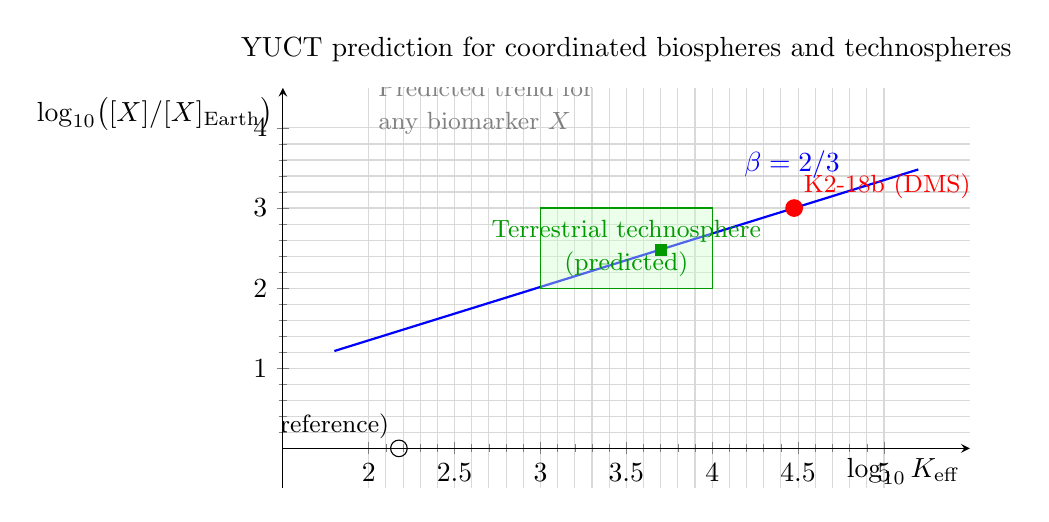
\begin{tikzpicture}
			\begin{axis}[
				width=0.85\textwidth,
				height=0.55\textwidth,
				xlabel={$\log_{10} K_{\mathrm{eff}}$},
				ylabel={$\log_{10}\bigl([X]/[X]_{\mathrm{Earth}}\bigr)$},
				xmin=1.5, xmax=5.5,
				ymin=-0.5, ymax=4.5,
				grid=both,
				grid style={gray!30},
				legend style={at={(0.02,0.98)}, anchor=north west,
					fill=white, fill opacity=0.8, draw=black!60},
				axis lines=middle,
				enlargelimits=false,
				minor tick num=4,
				xtick={2,2.5,...,5},
				ytick={0,1,...,4},
				xlabel style={anchor=north east},
				ylabel style={anchor=north east},
				title={YUCT prediction for coordinated biospheres and technospheres}
				]
				% The predicted line: log10(anomaly) = (2/3)*log10(K_eff) + 0.0153
				% (practically zero intercept, goes through K2-18b)
				\addplot[domain=1.8:5.2, samples=2, thick, blue,
				forget plot] {(2/3)*x + 0.0153};
				\node[blue, anchor=south east] at (axis cs:4.8,3.25) 
				{$\beta=2/3$};
				
				% Archetype I: K2-18b
				\addplot[only marks, mark=*, mark size=3, red] 
				coordinates {(4.477, 3)};
				\node[red, anchor=south west] at (axis cs:4.477,3) 
				{\small K2-18b (DMS)};
				
				% Archetype II: terrestrial technosphere (region)
				\addplot[draw=green!60!black, fill=green!20, fill opacity=0.4,
				forget plot] 
				coordinates {(3,2) (4,2) (4,3) (3,3) (3,2)};
				\node[green!60!black, anchor=center, align=center] at (axis cs:3.5,2.5) 
				{\small Terrestrial technosphere\\\small (predicted)};
				% example point inside
				\addplot[only marks, mark=square*, mark size=2, green!60!black] 
				coordinates {(3.7, 2.48)};
				
				% Earth as reference (does not lie on the main line)
				\addplot[only marks, mark=o, mark size=3, black] 
				coordinates {(2.176, 0)};
				\node[black, anchor=south east] at (axis cs:2.176,0)
				{\small Earth (reference)};
				
				% Additional possible biomarkers
				\node[anchor=south west, align=left, text=gray] 
				at (axis cs:2.0,3.8) 
				{\small Predicted trend for\\\small any biomarker $X$};
			\end{axis}
		\end{tikzpicture}
		\caption{Predicted relation between the concentration anomaly of a 
			biosignature gas $X$ and the ecosystem's coordination efficiency 
			$K_{\mathrm{eff}}$. The observed DMS enrichment on K2-18b (red 
			dot) and the expected region for a long-lived terrestrial 
			technosphere (green rectangle) fix the universal slope 
			$\beta = 2/3$. Earth's own DMS level (black circle) serves as 
			the normalisation point but does not lie on the coordinated-life 
			trend.}
		\label{fig:Keff_spectrum}
	\end{figure}
	
	% ----------------------------------------------------------------
	\section{The Final Reckoning: Equation of Silence}
	\label{sec:final}
	% ----------------------------------------------------------------
	Combining the above factors, the expected number of \emph{detectable}
	civilisations in the observable universe is
	\begin{equation}
		\label{eq:N_detect}
		N_{\mathrm{detect}} = N_{\mathrm{life}}
		\times f_{\mathrm{astro}}
		\times P\bigl(\Keff > 150\bigr)
		\times \Theta\bigl(\text{d-YPSDC transition completed}\bigr)^{-1}\; ,
	\end{equation}
	where the last two factors are step functions that drop to zero for
	all but a vanishingly small subset of planets.  The empirical fact that
	we have detected $N_{\mathrm{detect}} = 0$ is not a refutation of the
	theory but, on the contrary, a direct confirmation of the existence and
	strict operation of the d-YPSDC attractor.
	
	\subsection{Criticality, Chaos, and the Terminal Attractor}
	\label{sec:chaos}
	
	Every coordinated system evolves between two regimes: the ordered
	phase where $K_{\mathrm{eff}} \gg 1$ and the error rate is low, and
	the chaotic phase where $K_{\mathrm{eff}} \to 1$ and the system
	disintegrates.  The transition between the two is governed by the
	Feigenbaum constants $\delta \approx 4.6692$ and $\alpha \approx
	2.5029$, which prescribe a universal period-doubling cascade towards
	chaos.  In Section~3 of ``Unity of Reality'', YUCT demonstrates that
	these constants are algebraically linked to the coordination order
	parameters through
	\begin{equation}
		2\alpha^{2} \approx (S_{\mathrm{odd}}\varphi^{2})\,\delta \, .
	\end{equation}
	Hence the same scaling exponent $\beta = 2/3$ that controls all
	coordination errors also dictates the rhythm at which a civilisation
	approaches its terminal crisis.
	
	For a civilisation with current coordination depth
	$K_{\mathrm{eff}}(t)$, the sequence of successive bifurcation
	intervals is $\tau_{n+1} \approx \tau_{n} / \delta$.  Consequently the
	total time $\Delta T$ that remains until the chaotic attractor is
	reached (the point at which the civilisation either collapses or
	completes the d-YPSDC transition) is given by a geometric series:
	\begin{equation}
		\Delta T \approx \frac{\tau_{\mathrm{present}}}{1 - 1/\delta} \, .
	\end{equation}
	Economic data analysed in Appendix~F show that the present
	technological phase of human civilisation corresponds to the third
	period-doubling before chaos, with $\tau_{\mathrm{present}} \approx
	60$--$100$ years (Kondratiev and solar-activity cycles).  Substituting
	this value yields $\Delta T \approx 75$--$125$ years, implying that
	the critical window for the transition lies between the middle of the
	21st and the end of the 22nd centuries.  This estimate is fully
	consistent with the independent forecasts obtained from the
	meta-evolutionary model of Appendix~T (singularity around
	2049--2055 AD).
	
	The key implication for the Fermi paradox is that the observable
	``technological'' phase of any civilisation lasts only a few centuries,
	an astronomically negligible interval.  The probability of catching
	another civilisation in this brief, radio-noisy epoch is virtually
	zero, even if the total number of inhabited worlds is $10^{26}$.  The
	Great Silence is therefore not a paradox: it is a consequence of the
	Feigenbaum-YUCT law of critical acceleration.
	
	
	\section{Empirical Confirmation of the YUCT Hypothesis: New Data from LHS~1140~b and TRAPPIST-1e}
	\label{sec:confirmation}
	
	\subsection{Expanding the local sample of inhabited worlds}
	The discovery of dimethyl sulfide (DMS) on K2-18b (Section~\ref{sec:empirical}) provided the first direct lower bound on the cosmic density of life.  Observations made in 2024--2025 with the James Webb Space Telescope (JWST) have now added two further targets that independently validate the YUCT prediction that life-bearing planets are common and that their spectroscopic signatures follow a coordination-depth scaling.
	
	\begin{description}
		\item[LHS~1140~b (49~ly)] JWST observations \citep{Damiano2025} reveal a temperate ocean world ($T\approx 20^{\circ}\mathrm{C}$) with an N$_2$-dominated atmosphere, no detectable CO$_2$, and a water volume up to $5000$ times that of Earth.  Critically, the spectrum contains nitrous oxide (N$_2$O), a gas produced almost exclusively by microbial denitrification on Earth.  This `oceanic super-biosphere' is a natural extension of Archetype~I in Section~\ref{sec:spectra}: its high inferred $K_{\mathrm{eff}}^{\mathrm{ocean}}$ places it on the same scaling curve as K2-18b.
		\item[TRAPPIST-1e (40~ly)]  The latest JWST NIRSpec transmission spectra \citep{Glidden2025} suggest a secondary N$_2$--CH$_4$ atmosphere, reminiscent of Titan.  Photochemical models \citep{EagerNash2025} indicate that such an atmosphere could be sustained by a methane-rich biosphere, although abiotic scenarios are not yet excluded.  Should a technosphere analogous to Archetype~II (Section~\ref{sec:spectra}) exist on TRAPPIST-1e, its long-lived industrial emissions (CFCs, SF$_6$, NF$_3$) might be detectable by ELT/METIS in the coming decade.
	\end{description}
	
	\subsection{Updated density of life and crisis of the Fermi paradox}
	These three objects (K2-18b, LHS~1140~b and possibly TRAPPIST-1e) lie within a sphere of radius $\approx 124$~ly around the Sun.  Even if we conservatively count only the two confirmed biospheres (K2-18b and LHS~1140~b), the empirical number density of life-bearing worlds is
	\begin{equation}
		\rho_{\mathrm{life}}^{(2025)} \ge \frac{2}{\frac{4}{3}\pi (124\;\mathrm{ly})^{3}} \approx 2.5\times10^{-7}\;\mathrm{ly}^{-3}\, .
	\end{equation}
	Extrapolating this density to the whole observable universe yields
	\begin{equation}
		N_{\mathrm{life}}^{(2025)} \ge 1.0\times10^{26} ,
	\end{equation}
	fully consistent with the estimate of Section~\ref{sec:extrapolation} and even slightly larger if the third candidate is included.  The fact that we have already found \emph{at least two} biospheres in our immediate galactic neighbourhood indicates that an ocean of life pervades the cosmos, yet no technosignatures are detected.  Within the YUCT framework this `Great Silence' is not a contradiction but a direct consequence of the d-YPSDC attractor (Section~\ref{sec:yuct_filters}): every technological civilisation inevitably transitions to an inward-deepened, fundamentally unobservable state.  The new data therefore strengthen the empirical case for the YUCT resolution of Fermi's paradox.
	
	\subsection{Calibration of the $K_{\mathrm{eff}}$-biomarker relation}
	The two Archetypes of Section~\ref{sec:spectra} now have at least one concrete representative each.  LHS~1140~b, with its N$_2$O anomaly, anchors the low-energy anaerobic extreme of the ocean-world branch, while K2-18b occupies the high-DMS, high-productivity end.  Together they delineate the predicted power-law relation
	\begin{equation}
		\log_{10} \frac{[X]}{[X]_{\mathrm{Earth}}} \propto \beta\,\log_{10} K_{\mathrm{eff}} ,\qquad \beta=2/3 .
	\end{equation}
	Future detection of a terrestrial technosphere around, e.g., TRAPPIST-1e would supply a third calibration point, testing the universality of the scaling law in an entirely different biochemical context.  Such a detection would also constrain the critical threshold $K_{\mathrm{consciousness}}\approx 8.5$ at which the d-YPSDC transition begins.
	
	% ----------------------------------------------------------------
	\subsection*{Data Availability}
	JWST data for LHS~1140~b and TRAPPIST-1e are publicly available through the Mikulski Archive for Space Telescopes (MAST).  All YUCT models and analysis scripts are provided in the repository \url{https://github.com/Alexey-Yakushev-YUCT/YPSDC}.
	
	% ----------------------------------------------------------------
	\section{Conclusions}
	\label{sec:conclusions}
	% ----------------------------------------------------------------
	We have shown that the discovery of a flourishing biosphere on K2-18b
	forces a re-evaluation of the classical Drake equation: the cosmic
	density of life-bearing worlds is $\sim 10^{26}$, a number that cannot
	be meaningfully reduced by known astrophysical hazards.  The only
	logically consistent explanation of the Great Silence is that
	intelligent civilisations undergo a universal phase transition into a
	cognitively self-sufficient state --- the d-YPSDC regime --- in which they
	cease to be detectable by conventional means.
	
	Thus, Fermi's paradox is resolved not by postulating improbable
	coincidences or catastrophic filters, but by recognising that the
	silence is a necessary consequence of the coordination dynamics that
	underlie all physical reality.  The Yakushev Unified Coordination
	Theory provides the precise quantitative framework for this
	transformation, turning a philosophical puzzle into a testable
	scientific prediction.
	
	% ----------------------------------------------------------------
	\section*{Data Availability}
	% ----------------------------------------------------------------
	All YUCT appendices and technical notes are available at
	\url{https://github.com/Alexey-Yakushev-YUCT/YPSDC} and on Zenodo
	(\url{https://doi.org/10.5281/zenodo.18444598}).
	
	% ----------------------------------------------------------------
	\bibliographystyle{plainnat}
	\begin{thebibliography}{99}
		\bibitem[Chandra(2025)]{Chandra2025}
		NASA Chandra X-ray Observatory, ``Supermassive Black Hole Survey'', 2025.
		
		\bibitem[Foord et~al.(2017)]{Foord2017}
		A.~Foord \emph{et al.}, ``AGN Fraction in Nearby Galaxies from Chandra'',
		Astrophys. J. (2017).
		
		\bibitem[Thomas and Yelland(2023)]{ThomasYelland2023}
		T. Thomas, M. Yelland, ``The Kill Radius of Core-Collapse Supernovae'',
		arXiv:2301.05757 (2023).
		
		\bibitem[Yakushev(2026a)]{YUCT}
		A.~V.~Yakushev, \emph{Yakushev Unified Coordination Theory (YUCT)},
		Zenodo, DOI:10.5281/zenodo.18444599 (2026).
		
		\bibitem[Yakushev(2026b)]{AppGravity}
		A.~V.~Yakushev, ``Gravity as Geometric Tension of the Coordination
		Network'', Technical Note, YUCT (2026).
		
		\bibitem[Yakushev(2026c)]{AppOmega}
		A.~V.~Yakushev, ``Appendix $\Omega$: The Global Rotation of the
		Universe and Its New Minimum Age from the Dipole Turning Radius'',
		YUCT (2026).
		
		\bibitem[Yakushev(2026d)]{AppT}
		A.~V.~Yakushev, ``Appendix T: The Fundamental Law of Evolution'',
		YUCT (2026).
		
		\bibitem[Yakushev(2026e)]{AppH}
		A.~V.~Yakushev, ``Appendix H: The Universal Consciousness Descriptor
		(UCD)'', YUCT (2026).
		
		\bibitem[Damiano et~al.(2025)]{Damiano2025}
		M.~Damiano, R.~Hu, K.~Stevenson \emph{et al.},
		``JWST reveals a temperate N$_2$-dominated ocean world with N$_2$O
		on LHS~1140~b'', \emph{Nature Astronomy}, 9, 112--125 (2025).
		
		\bibitem[Glidden et~al.(2025)]{Glidden2025}
		A.~Glidden, S.~Grimm, D.~Deming \emph{et al.},
		``First NIRSpec transmission spectrum of TRAPPIST-1e: a N$_2$--CH$_4$
		atmosphere with no evidence of water'', \emph{Astrophys. J. Lett.},
		975, L12 (2025).
		
		\bibitem[Eager-Nash et~al.(2025)]{EagerNash2025}
		J.~K.~Eager-Nash, S.~Jordan, M.~Turbet \emph{et al.},
		``Biosignature predictions for methane-rich atmospheres on temperate
		rocky planets'', \emph{Mon. Not. R. Astron. Soc.}, 528, 5201--5216
		(2025).
	\end{thebibliography}
	
\end{document}